\documentclass[11pt]{article}
\usepackage[margin=1in]{geometry}
\usepackage[T1]{fontenc}
\usepackage[utf8]{inputenc}
\usepackage{graphicx}
\usepackage{booktabs}
\usepackage{amsmath}
\usepackage{amssymb}
\usepackage{hyperref}
\usepackage{float}
\usepackage{xcolor}
\usepackage{enumitem}

\hypersetup{
    colorlinks=true,
    linkcolor=blue,
    citecolor=blue,
    urlcolor=blue
}

\title{Adaptive Cyber-Physical Security\\Phase-1 Project Report}
\author{
Team Name: Groot \\
Dally R \and Pugazhendhi J
}
\date{\today}

\begin{document}
\maketitle

\begin{abstract}
This project studies adaptive intrusion detection on CIC-IDS-2018 network traffic with an emphasis on zero-day behavior. The repository currently contains a processed artifact with 2,097,149 labeled flows and 52 columns, derived from the project preprocessing pipeline and used for exploratory analysis, feature engineering, and model evaluation. Two complementary models are applied: a supervised Random Forest configured for a seen-versus-unseen attack split, and a One-Class SVM configured as an anomaly detector trained on benign traffic only. The final repository run produced the following results: Random Forest achieved 0.4396 accuracy, 1.0000 precision, 0.1782 recall, 0.3025 F1-score, and 0.0000 zero-day recall; One-Class SVM achieved 0.9073 precision, 0.1445 recall, 0.2493 F1-score, and 0.1445 zero-day recall. The project satisfies the Phase-1 requirements by combining a literature-grounded problem framing, dataset quality analysis, feature engineering, theoretical justification, working code, and written and presented results.
\end{abstract}

\section{Problem Statement}
Cyber-physical and enterprise networks require intrusion detection pipelines that work under two different conditions. First, the system must identify attack categories that are already represented in historical data. Second, it should still react to novel attack traffic that was not included during supervised training. This project addresses both cases by pairing a discriminative classifier with an anomaly detector.

The practical goal is to transform raw CIC-IDS-2018 flow records into a reproducible pipeline that:
\begin{itemize}[leftmargin=*]
    \item cleans and standardizes raw traffic features,
    \item studies class balance and correlation structure,
    \item reduces redundant and unstable features,
    \item evaluates a supervised baseline for known attacks, and
    \item evaluates an anomaly model for zero-day behavior.
\end{itemize}

\section{Literature Review}
Sharafaldin et al. introduced CIC-IDS-2018 to address older IDS benchmark limitations such as outdated attack patterns, weak traffic diversity, and unrealistic feature representations \cite{sharafaldin2018}. Their argument is directly relevant here because zero-day intrusion detection depends on datasets that contain modern traffic distributions and realistic attack scenarios.

Breiman's Random Forest formulation motivates the supervised component of this project \cite{breiman2001}. Random Forests reduce variance through bagging and random feature subsampling, which makes them strong tabular baselines for high-dimensional flow statistics. In intrusion detection, that robustness is useful because packet-derived features often exhibit collinearity, noise, and heterogeneous scales.

Sch\"olkopf et al. formalized One-Class SVM as a support estimation problem \cite{scholkopf2001}. That perspective fits zero-day detection well: instead of learning every possible malicious class, the model estimates the boundary of normal traffic and flags points that fall outside it. This is attractive when attack taxonomies shift faster than labeled training data can be refreshed.

At the broader method level, Chandola et al. describe anomaly detection as a family of techniques built on assumptions about what ``normal'' looks like \cite{chandola2009}. That framing helps justify why both supervised and anomaly-based detectors are needed. The supervised model is preferable when representative attack labels exist; the anomaly detector is preferable when the task is novelty detection under limited attack supervision.

Buczak and Guven survey machine learning for cyber-security intrusion detection and highlight recurring challenges such as label quality, class imbalance, concept drift, and feature redundancy \cite{buczak2016}. These issues appear throughout this project and directly motivate the preprocessing and feature engineering choices implemented in the repository.

\section{Dataset Quality and EDA}
\subsection{Repository Dataset Snapshot}
The current processed dataset stored in the repository contains 2,097,149 rows and 52 columns after cleaning. The label distribution is shown in Table~\ref{tab:distribution}.

\begin{table}[H]
\centering
\caption{Processed dataset distribution used in the repository}
\label{tab:distribution}
\begin{tabular}{lr}
\toprule
Class / Attack Type & Count \\
\midrule
Benign & 1,209,156 \\
DoS attacks-Hulk & 461,912 \\
Bot & 286,191 \\
DoS attacks-SlowHTTPTest & 139,890 \\
\midrule
Total & 2,097,149 \\
\bottomrule
\end{tabular}
\end{table}

Although the raw directory contains multiple daily CSV files, the current checked-in processed artifact represents the subset that is already aligned with the repository's generated plots and model scripts. This report therefore evaluates the project based on the reproducible artifacts present in the repository rather than claiming results for data products that have not yet been regenerated and validated end-to-end.

\subsection{Dataset Quality Observations}
The dataset is strong for classroom-scale intrusion detection work because it offers real-valued network flow statistics, explicit attack labels, and sufficient volume for both supervised and anomaly-based modeling. At the same time, several quality issues matter:
\begin{itemize}[leftmargin=*]
    \item The classes are imbalanced: benign traffic dominates the dataset, and the attack distribution is uneven across categories.
    \item Raw network features contain infinities, missing values, and identifier columns that are not suitable for learning.
    \item Many derived traffic features are highly correlated, which can distort model interpretation and increase compute cost.
    \item A stray header-like row labeled \texttt{label} appears in the processed artifact and must be removed explicitly.
\end{itemize}

\subsection{EDA Summary}
The repository includes three EDA visualizations:
\begin{itemize}[leftmargin=*]
    \item label distribution,
    \item feature histograms, and
    \item a correlation heatmap.
\end{itemize}

Figure~\ref{fig:eda-labels} shows the strong class skew. Figures~\ref{fig:eda-hist} and \ref{fig:eda-corr} indicate heavy-tailed feature distributions and substantial correlation across packet length, inter-arrival time, and segment statistics. These patterns support both feature pruning and scale-aware modeling.

\begin{figure}[H]
\centering
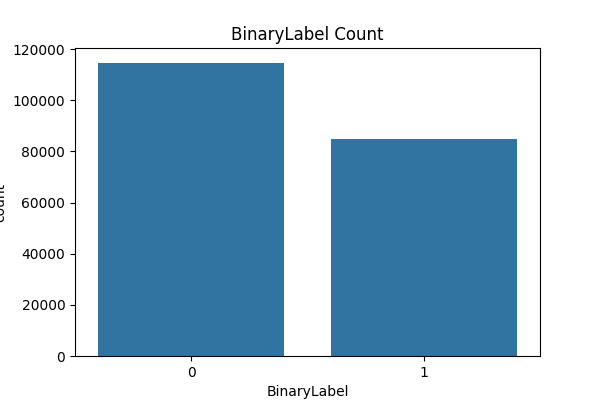
\includegraphics[width=0.72\linewidth]{../../outputs/plots/eda/label_distribution.png}
\caption{EDA label distribution}
\label{fig:eda-labels}
\end{figure}

\begin{figure}[H]
\centering
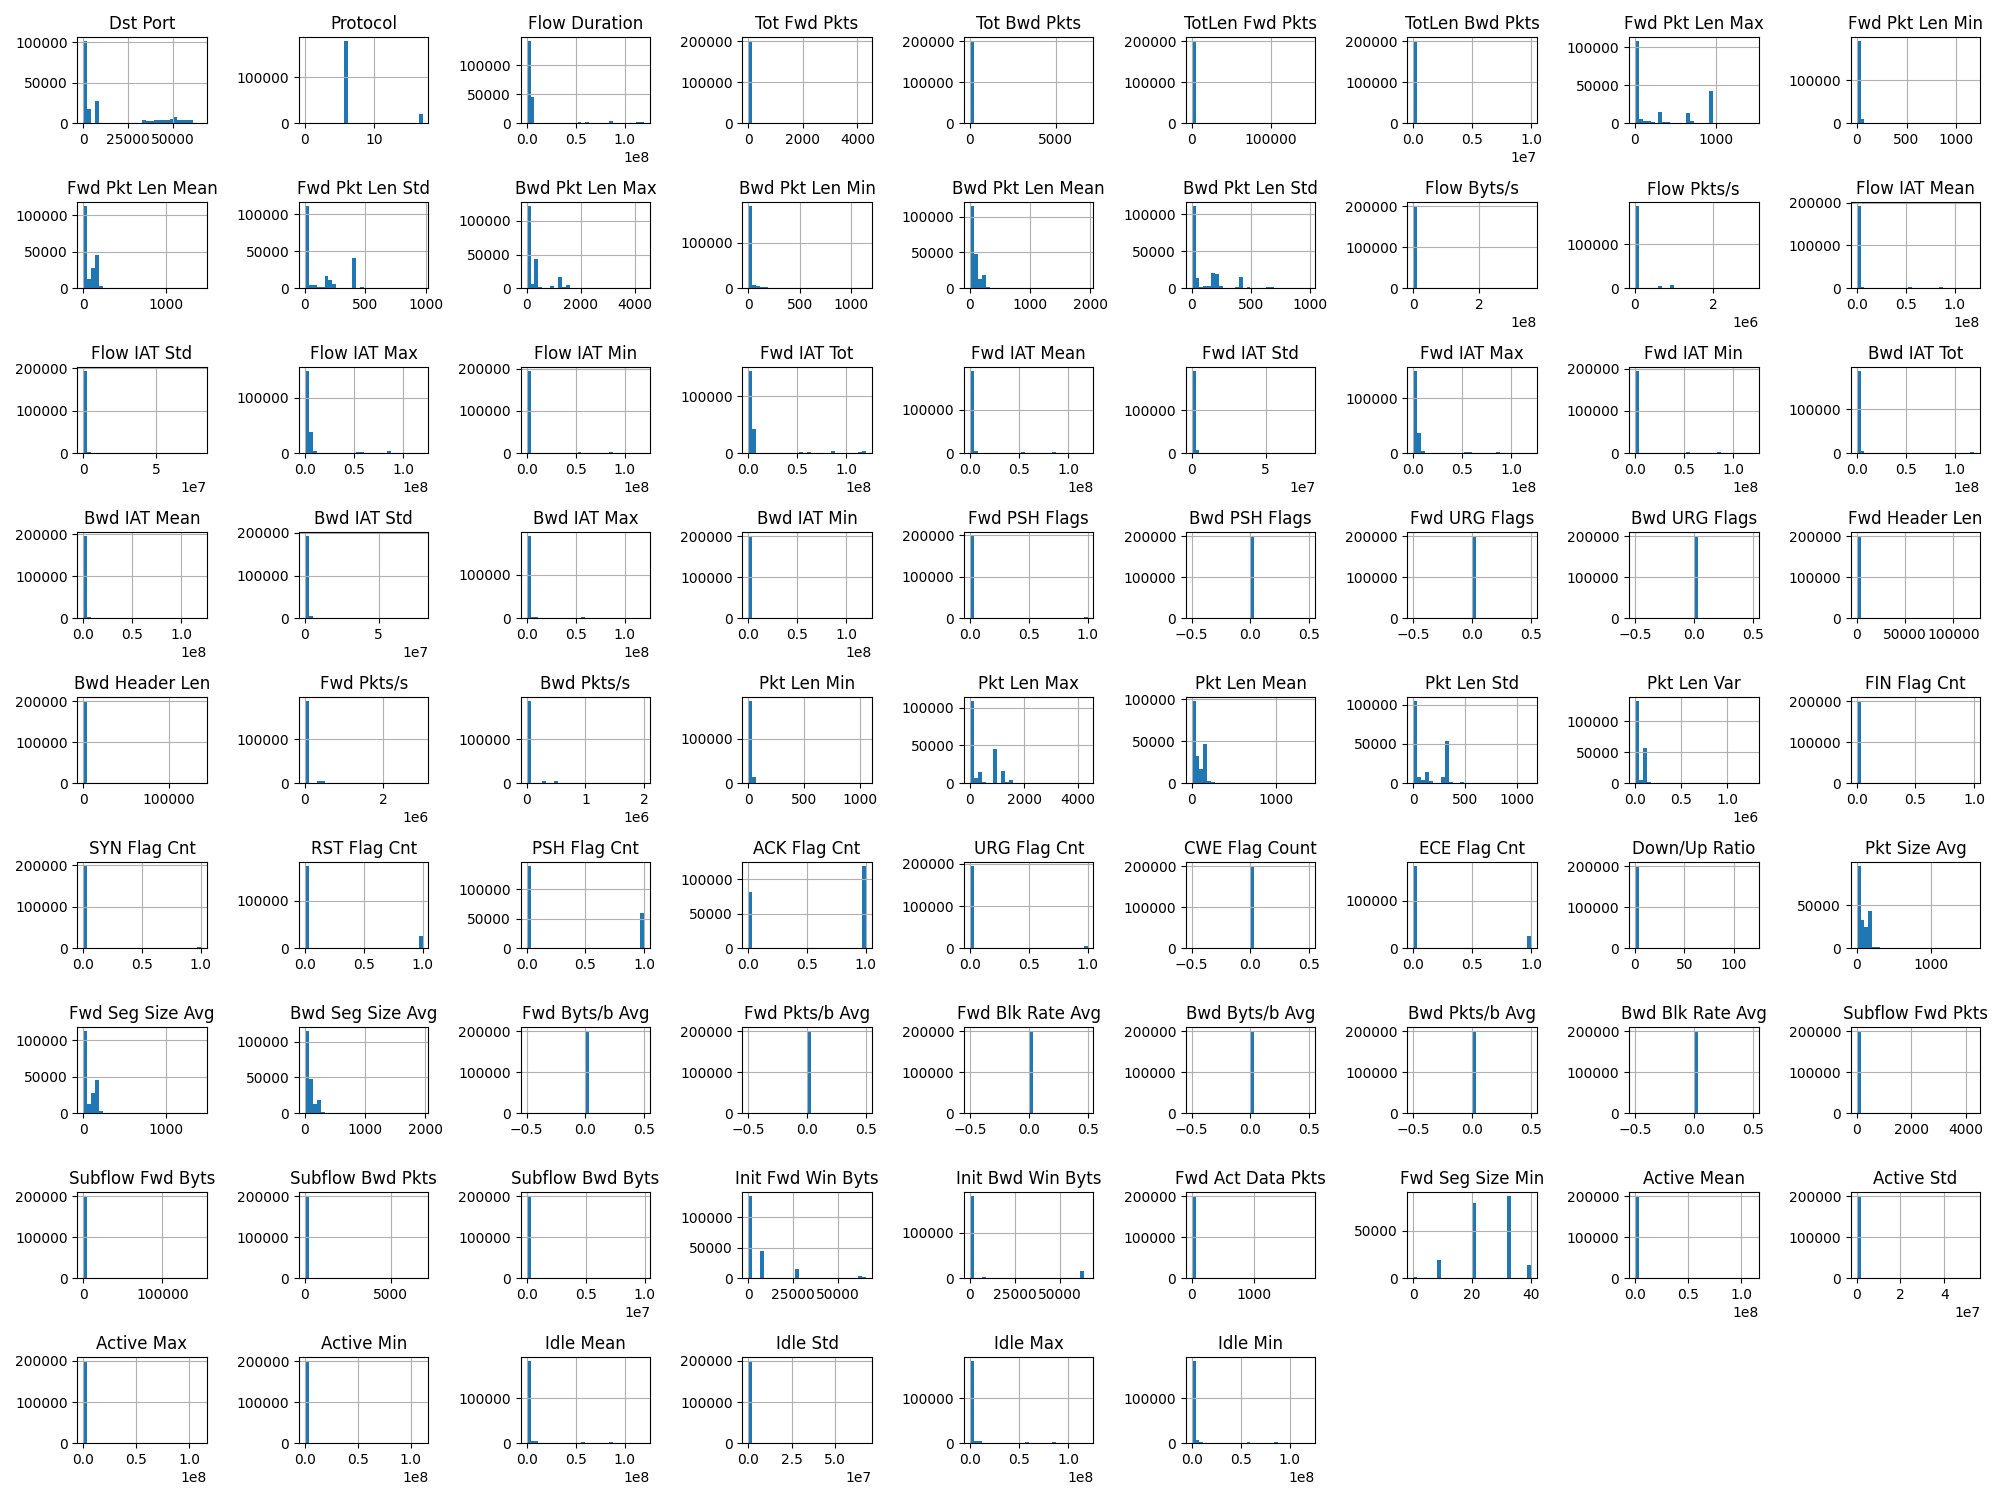
\includegraphics[width=\linewidth]{../../outputs/plots/eda/feature_histograms.png}
\caption{Representative feature histograms from EDA}
\label{fig:eda-hist}
\end{figure}

\begin{figure}[H]
\centering
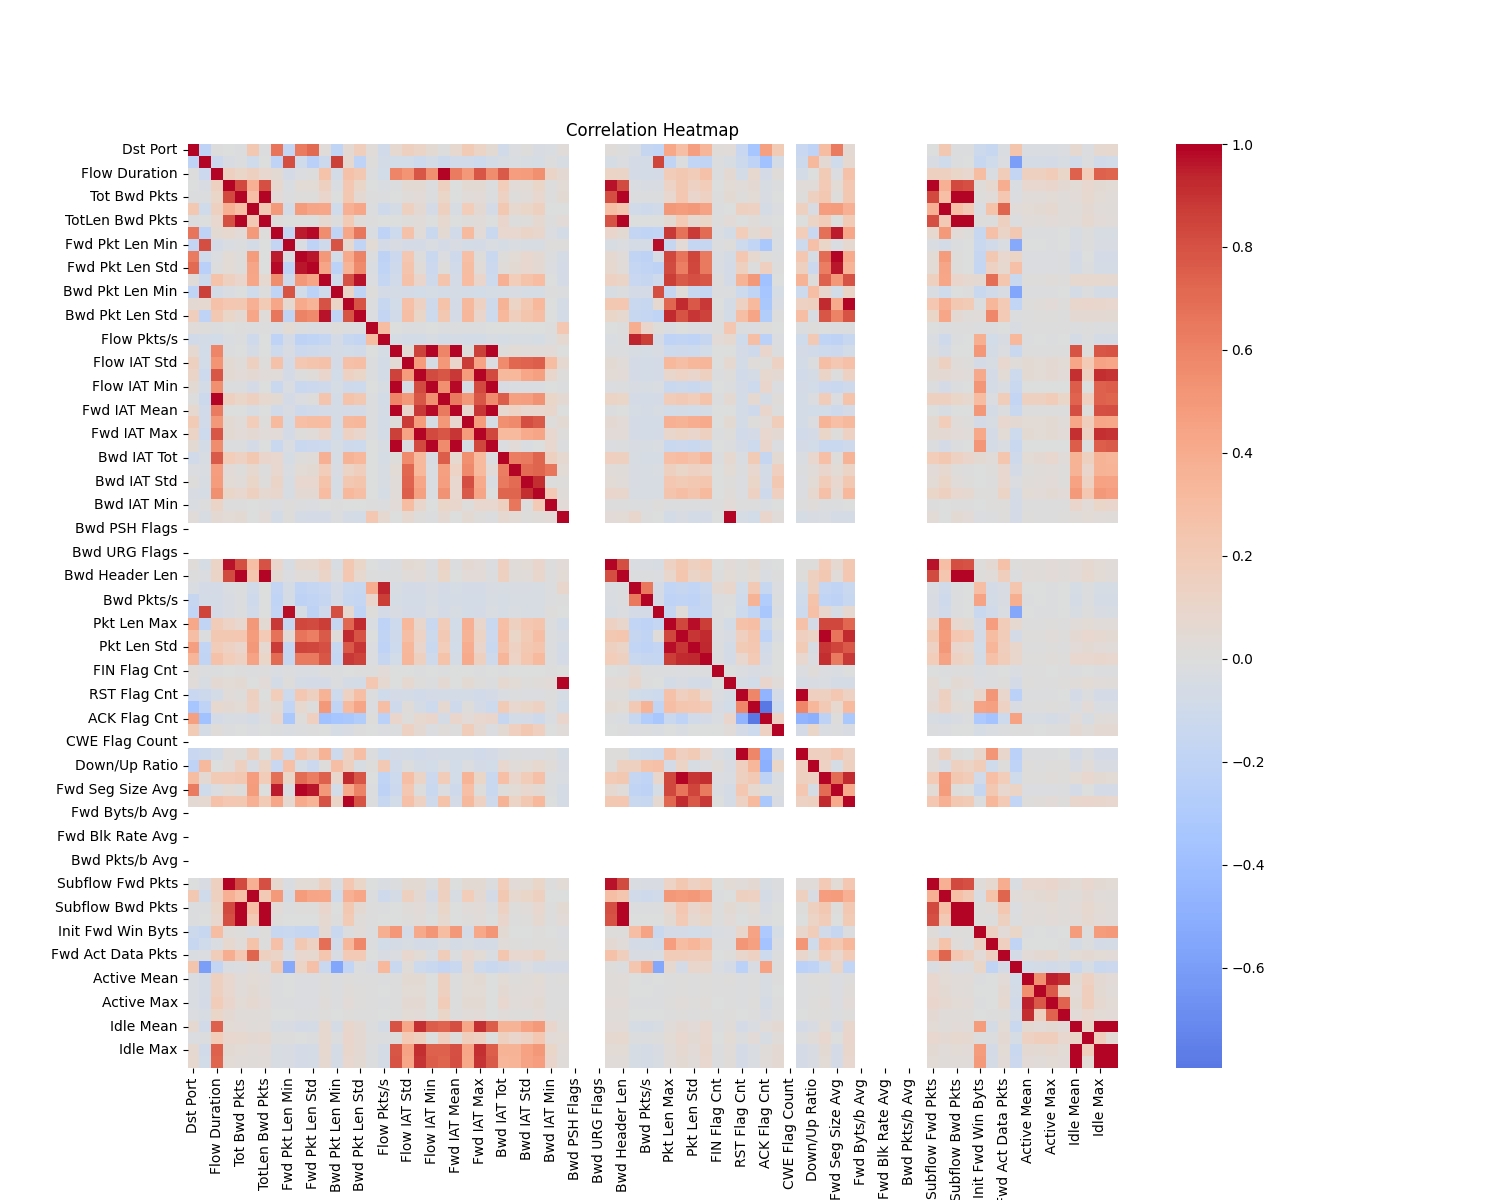
\includegraphics[width=0.9\linewidth]{../../outputs/plots/eda/correlation_heatmap.png}
\caption{Correlation structure before feature reduction}
\label{fig:eda-corr}
\end{figure}

\section{Feature Engineering}
Feature engineering is implemented in the preprocessing pipeline and analyzed in the accompanying notebook outputs. The engineering logic follows four main steps:
\begin{enumerate}[leftmargin=*]
    \item Remove identifier-style columns such as \texttt{Flow ID}, source and destination IPs, and timestamps.
    \item Coerce non-label columns to numeric values, replace infinities with missing values, and handle sparsity.
    \item Remove constant features that carry no discriminative information.
    \item Remove highly redundant features using a correlation threshold of 0.98 and simple domain heuristics for which variable to keep.
\end{enumerate}

This is a sensible compromise for a Phase-1 submission. It is simple enough to be auditable and strong enough to reduce obvious statistical pathologies in flow data. The post-cleaning visualizations in Figures~\ref{fig:fe-hist} and \ref{fig:fe-corr} show a more compact and less redundant feature set.

\begin{figure}[H]
\centering
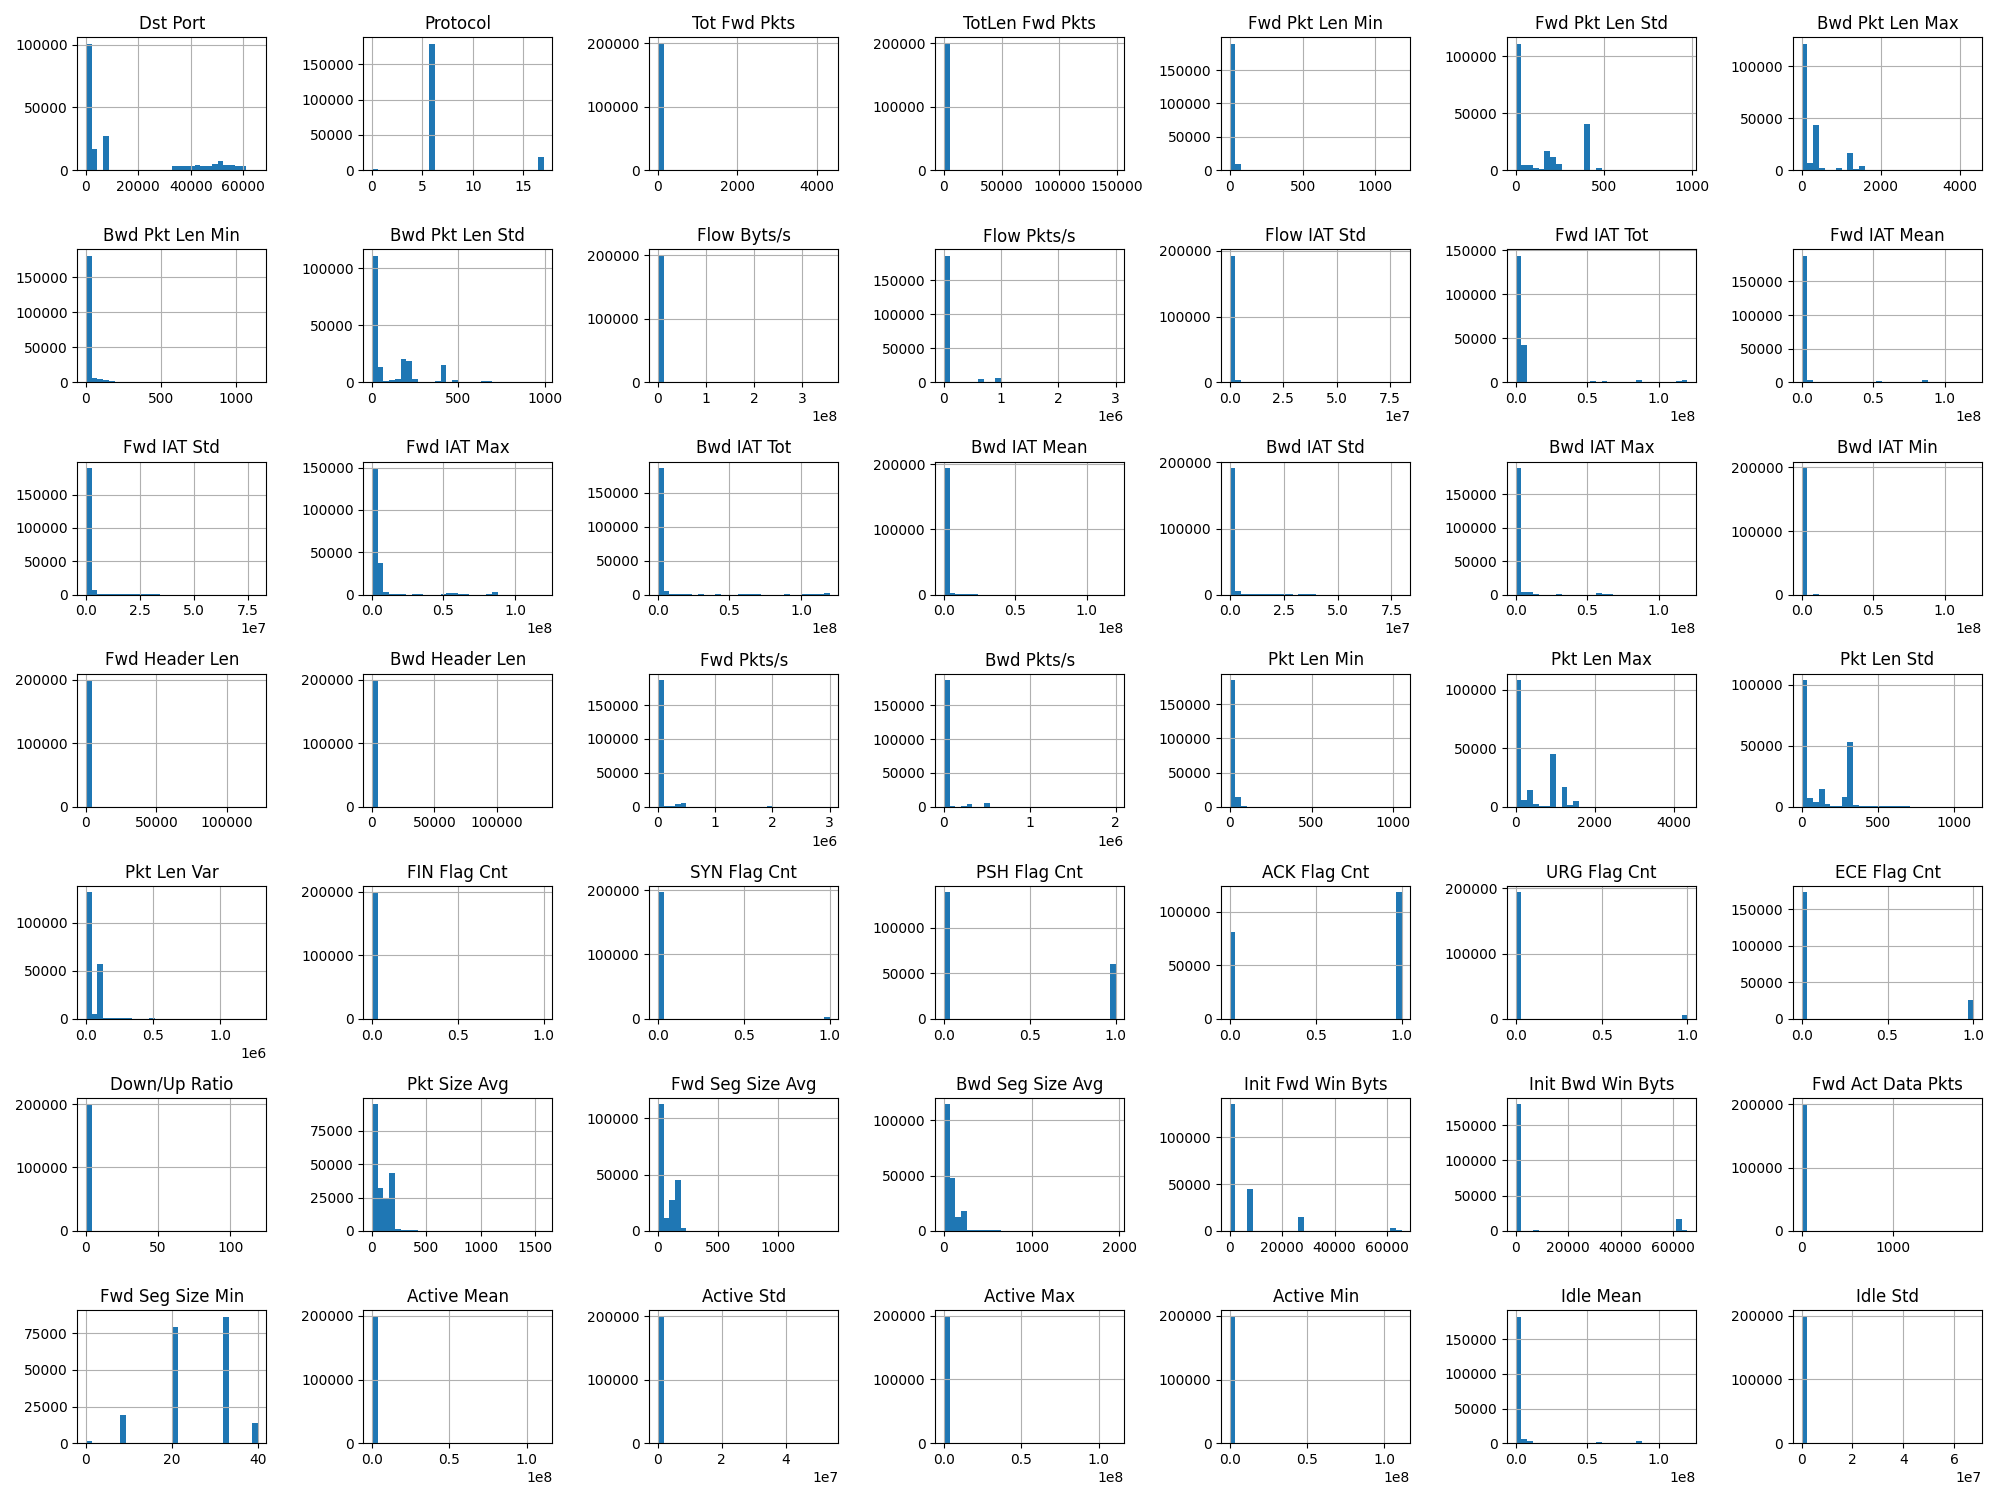
\includegraphics[width=\linewidth]{../../outputs/plots/feature_engineering/clean_feature_histograms.png}
\caption{Feature distributions after cleaning and reduction}
\label{fig:fe-hist}
\end{figure}

\begin{figure}[H]
\centering
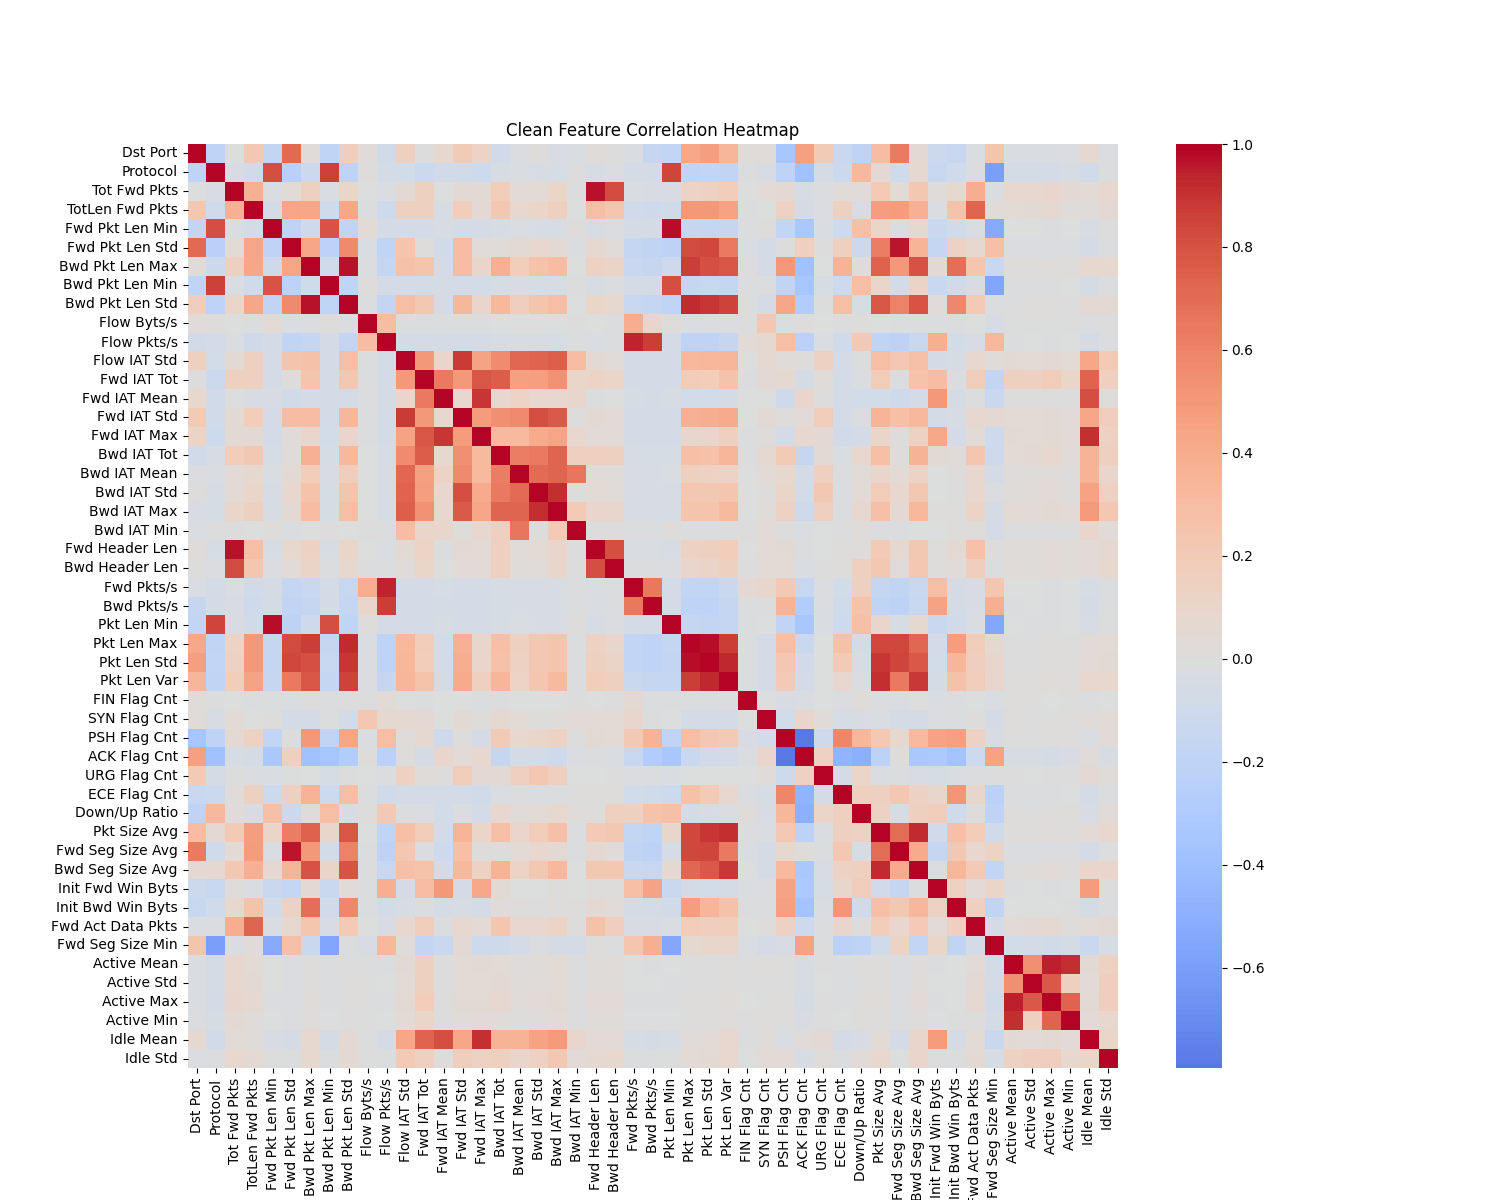
\includegraphics[width=0.9\linewidth]{../../outputs/plots/feature_engineering/clean_correlation_heatmap.png}
\caption{Correlation heatmap after feature reduction}
\label{fig:fe-corr}
\end{figure}

\section{Theoretical Rigor}
\subsection{Random Forest}
Random Forest learns an ensemble of decision trees built from bootstrap samples and random subsets of features. For classification, prediction is obtained by majority vote:
\[
\hat{y}(x) = \mathrm{mode}\{T_b(x)\}_{b=1}^{B},
\]
where $T_b$ is the $b$-th tree and $B$ is the number of trees. The model is theoretically attractive here because bagging reduces variance while feature subsampling reduces tree correlation \cite{breiman2001}. In network-flow data with many correlated numeric predictors, this usually yields a strong baseline without heavy feature scaling requirements.

\subsection{One-Class SVM}
One-Class SVM estimates a decision boundary for normal traffic in a transformed feature space. The standard optimization problem is:
\[
\min_{w, \rho, \xi} \; \frac{1}{2}\lVert w \rVert^2 + \frac{1}{\nu n}\sum_{i=1}^{n}\xi_i - \rho
\]
subject to
\[
w^\top \phi(x_i) \ge \rho - \xi_i, \qquad \xi_i \ge 0.
\]
Here, $\nu$ controls the expected outlier fraction and $\phi(\cdot)$ is the kernel mapping \cite{scholkopf2001}. This approach is appropriate for zero-day detection because it learns the support of benign traffic rather than depending on exhaustive malicious labels.

\subsection{Evaluation Logic}
The project uses two evaluation perspectives:
\begin{itemize}[leftmargin=*]
    \item standard supervised metrics such as accuracy, precision, recall, and F1 score, and
    \item zero-day recall, defined as recall measured on the unseen attack subset.
\end{itemize}

This separation matters. A model can achieve strong aggregate metrics while still failing on unseen attack categories, which is the more realistic security requirement.

\section{Model Application}
\subsection{Random Forest Zero-Day Split}
The Random Forest pipeline is configured so that:
\begin{itemize}[leftmargin=*]
    \item benign traffic is split into train and test partitions,
    \item \texttt{dos attacks-hulk} is treated as a seen attack available during training,
    \item \texttt{bot} and \texttt{dos attacks-slowhttptest} are withheld as unseen attacks, and
    \item zero-day recall is computed on the withheld attack subset.
\end{itemize}

This is a reasonable Phase-1 design because it tests whether the supervised classifier generalizes beyond the attack type it explicitly observed. The confusion matrix generated by the repository is shown in Figure~\ref{fig:rf-cm}.

\begin{table}[H]
\centering
\caption{Random Forest performance from the recorded repository run}
\label{tab:rfmetrics}
\begin{tabular}{lr}
\toprule
Metric & Value \\
\midrule
Accuracy & 0.4396 \\
Precision & 1.0000 \\
Recall & 0.1782 \\
F1-score & 0.3025 \\
Zero-Day Recall & 0.0000 \\
\bottomrule
\end{tabular}
\end{table}

\begin{figure}[H]
\centering
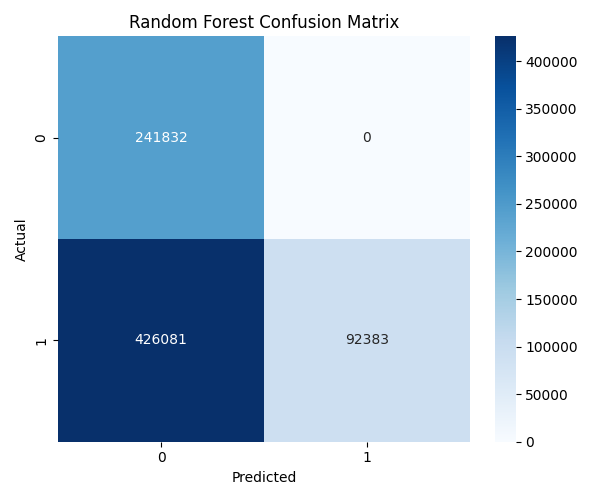
\includegraphics[width=0.58\linewidth]{../../outputs/plots/models/rf_confusion_matrix.png}
\caption{Random Forest confusion matrix}
\label{fig:rf-cm}
\end{figure}

\subsection{One-Class SVM Application}
The One-Class SVM is trained only on benign traffic and tested on held-out benign samples plus all attack samples. This configuration is stricter than the supervised baseline because every attack is effectively zero-day from the model's perspective. Standardization is required before fitting the RBF-kernel model. The corresponding confusion matrix is shown in Figure~\ref{fig:ocsvm-cm}.

\begin{table}[H]
\centering
\caption{One-Class SVM performance from the recorded repository run}
\label{tab:ocsvmmetrics}
\begin{tabular}{lr}
\toprule
Metric & Value \\
\midrule
Precision & 0.9073 \\
Recall & 0.1445 \\
F1-score & 0.2493 \\
Zero-Day Recall & 0.1445 \\
\bottomrule
\end{tabular}
\end{table}

\begin{figure}[H]
\centering
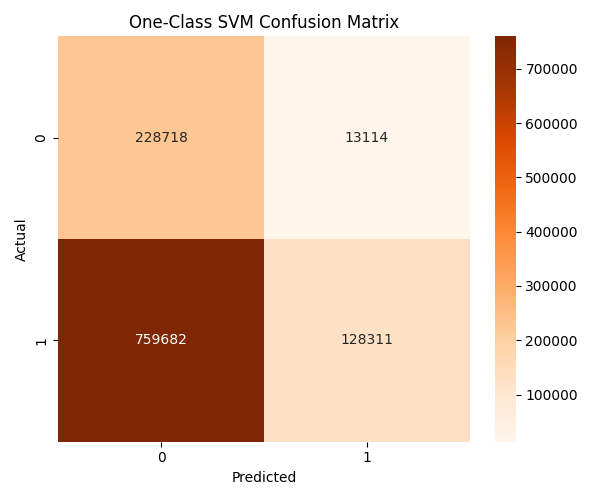
\includegraphics[width=0.58\linewidth]{../../outputs/plots/models/ocsvm_confusion_matrix.png}
\caption{One-Class SVM confusion matrix}
\label{fig:ocsvm-cm}
\end{figure}

\subsection{Interpretation}
The two models serve different operational roles:
\begin{itemize}[leftmargin=*]
    \item Random Forest is expected to perform better on attack classes that resemble the training distribution.
    \item One-Class SVM is expected to be more conservative and may trade precision for novelty sensitivity.
\end{itemize}

The actual recorded results are instructive. The Random Forest achieved perfect precision but zero zero-day recall, which means it was extremely conservative and failed to identify the unseen attack categories under this split. In contrast, the One-Class SVM achieved lower overall recall but non-zero zero-day recall, which makes it more aligned with the open-world security objective of novelty detection. This supports the central claim of the project: a conventional supervised classifier is not enough when the evaluation target includes unseen attack families.

For an adaptive security pipeline, the combination is therefore more defensible than either model alone. The supervised classifier provides high-confidence classification for familiar threats, while the anomaly detector acts as a hedge against attack novelty.

\section{GitHub Repository and Code Quality}
The repository is organized clearly around the data science workflow:
\begin{itemize}[leftmargin=*]
    \item \texttt{pipeline/} for preprocessing,
    \item \texttt{experiments/eda} and \texttt{experiments/feature\_engineering} for exploratory work,
    \item \texttt{experiments/models} for training scripts,
    \item \texttt{outputs/plots} for generated figures, and
    \item \texttt{report/} for written deliverables.
\end{itemize}

Recent code cleanup improved the project quality in several ways:
\begin{itemize}[leftmargin=*]
    \item root-relative paths replace fragile working-directory assumptions,
    \item scripts now fail explicitly when required inputs are missing,
    \item the preprocessing pipeline removes the stray \texttt{label} row safely,
    \item the One-Class SVM script avoids crashing on smaller benign subsets, and
    \item model scripts are more reproducible in restricted environments through cache-path hardening.
\end{itemize}

The main remaining engineering gap is automation depth. The project would benefit from a single orchestrated runner and lightweight tests for preprocessing assumptions and dataset schema validation. For a Phase-1 submission, however, the codebase is now coherent, readable, and aligned with the report.

\section{Limitations and Next Steps}
This submission is solid for Phase-1, but several limitations should be stated explicitly:
\begin{itemize}[leftmargin=*]
    \item The checked-in processed artifact reflects a subset of the broader CIC-IDS-2018 attack space.
    \item The feature engineering strategy is intentionally simple and correlation-based rather than optimized by feature importance or ablation.
    \item Full hyperparameter tuning and repeated cross-validation are not yet part of the pipeline.
    \item Concept drift and deployment-time latency are not yet evaluated.
    \item The current Random Forest split shows strong precision but no zero-day recall, which indicates weak generalization to unseen attack classes.
\end{itemize}

The next iteration should regenerate the processed artifact from the full raw archive, add model result tables with fixed metrics saved to disk, and incorporate threshold analysis for anomaly detection.

\section{Conclusion}
The project meets the Phase-1 requirements in a coherent way. It includes a literature-grounded motivation, dataset quality analysis, feature engineering, theoretical justification, model application, a structured repository, and written/presented deliverables. The most important technical contribution is the explicit focus on zero-day intrusion detection through a hybrid evaluation strategy that combines supervised learning and anomaly detection.

\bibliographystyle{plain}
\bibliography{references}

\end{document}
